%; whizzy paragraph -pdf xpdf -latex ./whizzypdfptex.sh
%; whizzy-paragraph "^\\\\begin{frame}"
% latex beamer presentation.
% platex, latex-beamer でコンパイルすることを想定。 

%     Tokyo Debian Meeting resources
%     Copyright (C) 2009 Junichi Uekawa
%     Copyright (C) 2009 Nobuhiro Iwamatsu

%     This program is free software; you can redistribute it and/or modify
%     it under the terms of the GNU General Public License as published by
%     the Free Software Foundation; either version 2 of the License, or
%     (at your option) any later version.

%     This program is distributed in the hope that it will be useful,
%     but WITHOUT ANY WARRANTY; without even the implied warreanty of
%     MERCHANTABILITY or FITNESS FOR A PARTICULAR PURPOSE.  See the
%     GNU General Public License for more details.

%     You should have received a copy of the GNU General Public License
%     along with this program; if not, write to the Free Software
%     Foundation, Inc., 51 Franklin St, Fifth Floor, Boston, MA  02110-1301 USA

\documentclass[cjk,dvipdfmx,12pt]{beamer}
\usetheme{Tokyo}
\usepackage{monthlypresentation}
\usepackage{listings}

%  preview (shell-command (concat "evince " (replace-regexp-in-string "tex$" "pdf"(buffer-file-name)) "&")) 
%  presentation (shell-command (concat "xpdf -fullscreen " (replace-regexp-in-string "tex$" "pdf"(buffer-file-name)) "&"))
%  presentation (shell-command (concat "evince " (replace-regexp-in-string "tex$" "pdf"(buffer-file-name)) "&"))

%http://www.naney.org/diki/dk/hyperref.html
%日本語EUC系環境の時
\AtBeginDvi{\special{pdf:tounicode EUC-UCS2}}
%シフトJIS系環境の時
%\AtBeginDvi{\special{pdf:tounicode 90ms-RKSJ-UCS2}}

\title{.debから Python パッケージへの変遷}
\subtitle{}
\author{まえだこうへい}
\date{2015年4月18日}
\logo{
\includegraphics[width=8cm]{image200607/openlogo-light.eps}}

\begin{document}
\lstset{ %
  backgroundcolor=\color{dancerlightblue},
  language=sh
}

\frame{\titlepage{}}

\begin{frame}{自己紹介(2014年4月の時)}
 \begin{itemize}
  \item[Debian:] blockdiagシリーズ、django REST framework、\\yrmcdsなどのメンテナ
  \item[言語:] 主にPython。\\最近Golangも使おうと勉強中
  \item[家庭:] 猫一匹(♀)、娘二人、妻一人
  \item[勉強会:] ほぼDebian勉強会のみ。でも今日は約半年ぶり
  \item[仕事:] PythonでLDAPごにょごにょとか、\\django REST frameworkでAPI開発とか
 \end{itemize}
\end{frame}

\begin{frame}{自己紹介(今回)}
 \begin{itemize}
  \item[Debian:] blockdiagシリーズ、django REST framework、\\yrmcdsなどのメンテナ
  \item[言語:] 仕事はPython。PrivateはGolang。\\最近C++勉強始めました
  \item[家庭:] 猫一匹(♀)、娘二人、妻一人
  \item[勉強会:] ほぼDebian勉強会のみ。でも今回も約9ヶ月ぶり\footnote{前回の時はプレゼン資料作り忘れました}
  \item[仕事:] Private CloudのController(IaaS)\\のメンテを引き継ぎ中
 \end{itemize}
\end{frame}

\begin{frame}{今日の話の流れ}
  \begin{itemize}
  \item 今回のお話の背景
  \item ローカル Debian CIのおさらい
  \item ローカル Python CI (New!)
  \item before / after
  \item PythonパッケージはDebianパッケージにすべきか?
\end{itemize}
\end{frame}

\begin{frame}
  \begin{center}
    {\Huge シリーズ物の第三弾\\三年がかりで最終回(違}
  \end{center}
\end{frame}

\begin{frame}{開発、PythonとDjangoに統一するってよ}

  え、今頃…?(2014年9月現在)\footnote{本日現在諸事情により更にOpenStack導入に方針に変わっています}
  \begin{itemize}
  \item プロジェクトの開始当初から2年半
  \item Python以外でJavaとかGolangで開発したユーティリティも増えました
  \item PythonのWebフレームワークも開発初期はDjango以外にFlaskも使ってました
  \item 最初のリリース後増員された人員も、減っていく一方
  \end{itemize}

\end{frame}

\begin{frame}{組織人員の構成}

  \begin{tabular}{|l|c|}
    \hline
    属性 & おおよその比率 \\
    \hline
    プログラミングできない人 & 6割\footnote{うちPythonお勉強中の人は5割} \\
    JavaやRubyでは開発できる & 3割 \\
    Djangoを使ったことがない & 8割 \\
    {\scriptsize django REST framework}を使ったことが無い & 9割 \\
    Pythonでユニットテスト書いたことが無い & 私以外全員 \\
    Pythonパッケージを作ったことがない & 私以外全員 \\
    \hline
  \end{tabular}

  なんらかの方法で下駄を履かせないといけませんでした

\end{frame}

\begin{frame}{下駄を履かせるために行ったこと}

  {\footnotesize
  \begin{itemize}
  \item 開発標準の方針の文書化
  \item Pythonパッケージ用テンプレートの作成 \\
    {\tiny
      文法チェック/ユニットテスト/カバレッジ計測を強制実行, ドキュメント自動生成, Pythonパッケージ作成, Gitリポジトリ作成・設定など}
  \item Django用Pythonパッケージのテンプレート作成 \\
    {\tiny 各種ベストプラクティス適用, django REST frameworkの適用, サンプルアプリの提供など}
  \item 独自認証システム\footnote{この時の開発スコープの一コンポーネント}用のライブラリ開発 \\
    {\tiny 本番環境と開発用のモックモードの切替機能, Django認証モジュールの開発, 前述のテンプレートへの組み込みなど}
  \item Pythonパッケージ用のローカルリポジトリ(ローカルPyPI)の構築
  \item Jenkinsでの関連システムの統合(ローカルPyPI CI) \\
    {\tiny GitHub:e, テスト自動実行, HipChatへの通知, ローカルPyPIへのアップロードなど}
  \item 説明会、アップデートの通知、個別フォロー
  \end{itemize}
  }
\end{frame}

\begin{frame}{その前におさらい。ローカルDebian CI}
  Jenkinsで、ソースパッケージからビルド、テスト、ローカルアーカイブにアップロードする仕組み
\end{frame}

\begin{frame}{ローカルPyPI CI}
  Jenkinsで、Gitリポジトリからユニットテスト、ローカルPyPIにアップロードする仕組み
\end{frame}

\begin{frame}{比較}
  機能的にほぼ同じ+α
  \begin{center}
    {\scriptsize
  \begin{tabular}{|l|c|c|}
    \hline
    機能 & ローカルDebian CI & ローカルPyPI CI \\
    \hline
    ミラー & apt-mirror & bandersnatch \\
    リポジトリ & GitHub:e & GitHub:e or 公式ミラーなど \\
    ジョブスクリプト & Pythonで実装 & Pythonで実装 \\
    クリーン(ビルド)環境 & cowbuilder & virtualenv \\
    テスト & lintian, piuparts & tox \\
    署名 & pydebsign & n/a \\
    アップロード & dput & devpi client \\
    ローカルアーカイブ/リポジトリ & reprepro & devpi server \\
    パッケージテンプレート & n/a & シェルスクリプトで実装 \\
    Git push /pull request hook & n/a & GitHub:e webhook \\
    テスト結果通知 & n/a & HipChat \\
    \hline
  \end{tabular}}
  \end{center}
\end{frame}

\begin{frame}{比較}
  \begin{minipage}[t]{0.49\hsize}
    ローカルDebian CI
    \begin{figure}[H]
      \begin{center}
        \includegraphics[width=1.1\hsize]{image201504/debian-ci.eps}
      \end{center}
    \end{figure}
  \end{minipage}
    \begin{minipage}[t]{0.49\hsize}
    ローカルPyPI CI
    \begin{figure}[H]
      \begin{center}
        \includegraphics[width=1.1\hsize]{image201504/python-ci.eps}
      \end{center}
    \end{figure}
  \end{minipage}
\end{frame}

\begin{frame}{.debからPythonパッケージへのBefore/After}
  Debianのカスタムビルドパッケージとの比較の話。
  \begin{itemize}
  \item パッケージ化を行えるメンバーの増加
  \item 開発時のリポジトリ切替の簡易化
  \item パッケージ化のコスト削減
  \end{itemize}
  ※開発標準化のbefore/afterの話ではありません
\end{frame}

\begin{frame}

  {\Huge PythonパッケージはDebianパッケージにすべきか?}
  
\end{frame}

\begin{frame}{したほうが良い}
  \begin{itemize}
  \item システムグローバルでインストールするツール\footnote{\texttt{sudo pip install}とするケース}
  \item PyPIで公開されてないC bindingのライブラリ
  \end{itemize}
\end{frame}

\begin{frame}{しても良い}
  \begin{itemize}
  \item コマンドラインツール
  \item デーモン
   \item PyPIで公開されているC bindingのライブラリ
  \end{itemize}
\end{frame}

\begin{frame}{しなくても良い}
  \begin{itemize}
  \item DebianパッケージではないPythonパッケージに依存されないパッケージ
  \end{itemize}
\end{frame}

\begin{frame}{すると辛い}
  \begin{itemize}
    \item 開発が活発で、コマンドラインやデーモンにも依存されないライブラリ
  \end{itemize}
\end{frame}
  
\begin{frame}{まとめ}

  {\Huge ケースバイケース}
  
\end{frame}

\end{document}
